We generate $x=T\,u+N\,v+\varepsilon$ in $\mathbb{R}^{256}$ with unit vectors $u,v$ at a chosen cosine (``overlap''), binary $T$ and $N$ with training agreement $\rhot$, and anisotropic Gaussian noise (power-law spectrum). A nuisance edit is exact: $x'=x\pm v$. We fit the same extractors with the same code and compute $\cfn$ on a decorrelated pool. With no overlap, $\cfn$ grows with training correlation (from $\approx0$ at $\rhot=0.5$ to $\approx0.75$ at $0.9$) for every standard extractor: the familiar shortcut. With decorrelated training, $\cfn$ grows with overlap (by \synCFRangeStdMin--\synCFRangeStdMax{} across overlaps for standard extractors) while decodability changes relatively little (by at most \synDecRangeStd; \synDecRangeNe{} for the erased probe; Figure~\ref{fig:synth}). In this low signal-to-noise setting even logistic probes inherit the overlap; in CEBaB, where the target is decoded far better, they inherit much less of it (\S\ref{sec:results}). The synthetic setting illustrates that decodability is largely insensitive to overlap; it is not a model of the real representations.

\begin{figure}[h]
\centering
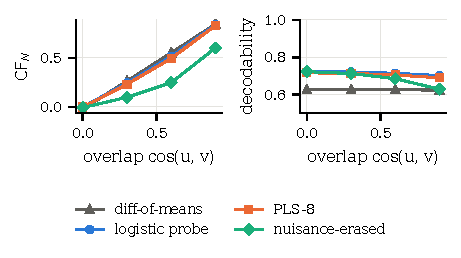
\includegraphics[width=\columnwidth]{figs/fig_synthetic.pdf}
\caption{Synthetic representation, decorrelated training ($\rhot=0.5$): nuisance sensitivity (left) and decodability (right) as target--nuisance overlap grows; means over 5 replicates.}
\label{fig:synth}
\end{figure}
